\documentclass[11pt]{article}
\usepackage[utf8]{inputenc}
\usepackage[russian]{babel}
\usepackage[T1]{fontenc}
\usepackage{amssymb,amsmath,clrscode,graphicx,indentfirst}

\author{Олег Смирнов}
\title{Курс kiev-clrs -- Лекция 8. Универсальное хэширование. Идеальное хэширование}
\date{23 мая 2009 г.}

\begin{document}
\maketitle
\tableofcontents

\newpage
\setlength{\parskip}{1ex plus 0.5ex minus 0.2ex}
\section{Цель лекции}
\begin{itemize}
\item Свойства и способ построения универсальных хэш-функций
\item Свойства идеального хэширования
\end{itemize}

\section{Универсальное хэширование}

Фундаментальная проблема хэширования заключается в том, что при любом выборе хэш-функции существует некоторый набор ключей, которые хэшируются в один и тот же слот таблицы.

Например, при разработке компилятора который использует хэш-таблицу для хранения имен переменных, возможно подготовить такой тестовой файл, что все имена попадут в один слот таблицы и это существенно замедлит компиляцию.

Идея: разработать метод выбора хэш-функции случайным образом, независимо от ключей. В этом случае будет невозможно использовать заранее заготовленный набор ``плохих'' ключей.

Определение: Пусть $U$ -- множество всех ключей и пусть $H$ -- конечное множество хэш-функций $f: U \to \{0, 1, \twodots, m-1\}$. Множество $H$ называется универсальным, если для любых $x, y \in U$, при $x \neq y$: $|\{h \in H:h(x) = h(y)\}| = |H|/m$. Т.е. шанс коллизии между ключами $x$ и $y$ будет $1/m$ (шанс попасть в розовую область на рисунке) для любого случайного выбора $h$ из $H$.
\begin{figure}[ht]
  \centering
  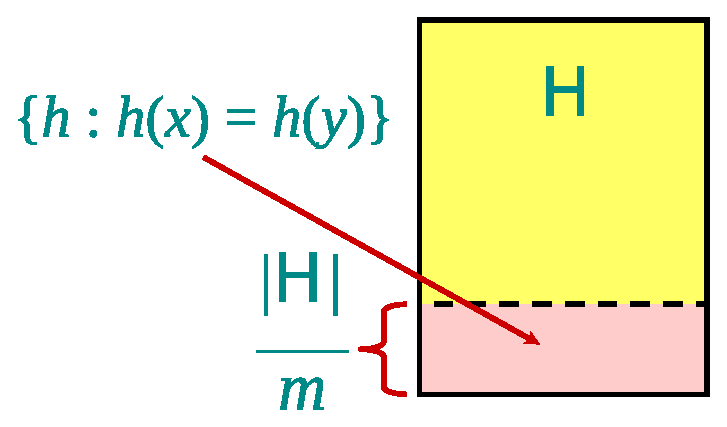
\includegraphics[width=3in]{lecture8/universal.eps}
  \caption{Универсальное хэширование}
  \label{fig:universal}
\end{figure}

Теорема: Пусть $h$ -- хэш-функция выбранная равновероятно из универсального множества $H$. Пусть функция $h$ используется для хэширования $n$ ключей в $m$ слотов таблицы $T$. Тогда для произвольного ключа $x$ выполняется $E[\#\text{коллизии с }x] < n/m = \alpha$.

Т.е. функции в универсальном множестве ведут себя в точности таким образом, как нам нужно.

Пусть $C_x$ -- случайная величина, показывающая количество коллизий в $T$ с ключем $x$ и пусть индикаторная случайная величина
\begin{equation*}
  C_{xy} = \begin{cases}
      1, \text{если } h(x) = h(y) \\
      0, \text{иначе}
  \end{cases}
\end{equation*}
Очевидно, что $E[C_{xy}] = 1/m$ и $C_x = \sum_{y \in T-\{x\}}C_{xy}$. Тогда
\begin{align*}
  E[C_x] = E\left[\sum_{y \in T-\{x\}}C_{xy}\right] = \\
  = \sum_{y \in T-\{x\}}\underbrace{E[C_{xy}]}_{\frac{1}{m}} = \\
  = \sum_{ \underbrace{y \in T-\{x\}}_{n-1} }\frac{1}{m} = \\
  = \frac{n-1}{m} < \frac{n}{m}
\end{align*}

\section{Конструкция универсального множества}

Пусть количество слотов в таблице $m$ -- простое число.

Идея: разложить ключ $k$ на $r+1$ цифр по основанию $m$, т.е. в промежутке $\{0, 1, \twodots, m-1\}$. Тогда $k = < k_0, k_1, \twodots k_r >$, где $0 \leqslant k_i \leqslant m$.

Вектор $a = <a_0, a_1, \twodots, a_r>$ состоит из элементов, выбранных случайно в промежутке ${0, 1, \twodots, m-1}$ независимо друг от друга. Таким образом существует $\prod_{i=0}^{r} m = m^{r+1}$ вариантов выбора.

Хэш-функция имеет вид:
\begin{equation*}
  h_a(k) = \left(\sum_{i=0}^{r} a_i k_i\right) \bmod m
\end{equation*}

Тогда $|H| = \{ h_a \} = m^{r+1}$

Теорема: Множество $H = \{h_a\}$ является универсальным.

Пусть $x = <x_0, x_1, \twodots, x_r>$ и $y = <y_0, y_1, \twodots, y_r>$ -- два различных ключа из множества $U$. Т.к. они различны, их разложения должны различаться хотя бы в одной цифре. Не теряя общности, можно предположить, что они различаются в первой цифре (с индексом 0). Необходимо, как часто выполняется условие коллизии:
\begin{align*}
  h_a(x) = h_a(y) \\
  \sum_{i=0}^r a_i x_i \equiv \sum_{i=0}^r a_i y_i (\bmod m) \\
  \sum_{i=0}^r a_i(x_i - y_i) \equiv 0 (\bmod m) \\
  \text{или} \\
  a_0(x_0-y_0) + \sum_{i=1}^r a_i x_i \equiv 0 (\bmod m) \\
  a_0(x_0-y_0) \equiv - \sum_{i=1}^r a_i x_i (\bmod m)
\end{align*}

Теорема: пусть $m$ -- простое число. Тогда для любого $z \in \mathbb{Z}_m$, такого, что $z \neq 0$, существует единственный элемент $z^{-1} \in \mathbb{Z}_m$, такой, что
\begin{equation*}
  z \cdot z^{-1} \equiv 1 (\bmod m)
\end{equation*}
Пример для $m = 7$.
\begin{figure}[ht]
  \centering
  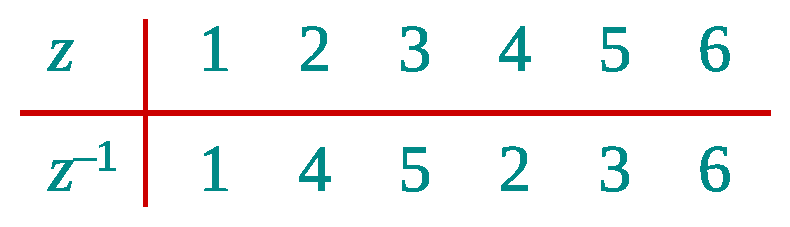
\includegraphics[width=3in]{lecture8/z7.eps}
  \caption{Кольцо вычетов $\mathbb{Z}_7$}
  \label{fig:z7}
\end{figure}

Итак, 
\begin{align*}
  a_0(x_0-y_0) \equiv - \sum_{i=1}^r a_i x_i (bmod m) \\
  \text{из факта } x_0 \neq y_0 \text{ и существования } (x_0 - y_0)^{-1} \\
  a_0 \equiv \left(-\sum_{i=1}^{r} a_i(x_i - y_i)\right)\cdot(x_0-y_0)^{-1} (\bmod m)
\end{align*}

Таким образом, для двух различных ключей, для всех возможных вариантов выбора элементов $a_1, a_2, \twodots, a_r$ существует только единственный вариант выбора элемента $a_0$, который реализует функцию $h_a$, дающую коллизию.

Т.е. существует $m$ вариантов выбора для $a_1, a_2, \twodots, a_r$ и один для $a_0$ (по приведенной формуле). Общее число функций $h_a$, дающих коллизию элементов $x$ и $y$ будет равно
\begin{equation*}
  m^r\cdot1 = m^r = \frac{|H|}{m}
\end{equation*}

\section{Идеальное хэширование}

Задача идеального хэширования возникает тогда, когда возникает необходимость проверять наличие элемента (скажем, слова из словаря) за гарантировано константное время. При этом подразумевается, что набор данных в таблице статичен либо изменяется очень редко.

Задача: для заданного набора из $|U| = n$ ключей создать статическую хэш-таблицу размера $m = O(n)$, такую что операция поиска Search выполнялась бы за $\Theta(1)$ в худшем случае. Таблица должна быть статической, т.е. операции добавления и удаления элементов в ней не поддерживаются.

Идея: сконструировать двухуровневое хэширование с универсальной хэш-функцией на каждом из уровней. Выбрать функции таким образом, чтоб обеспечить отсутствие коллизий на уровне 2.
\begin{figure}[ht]
  \centering
  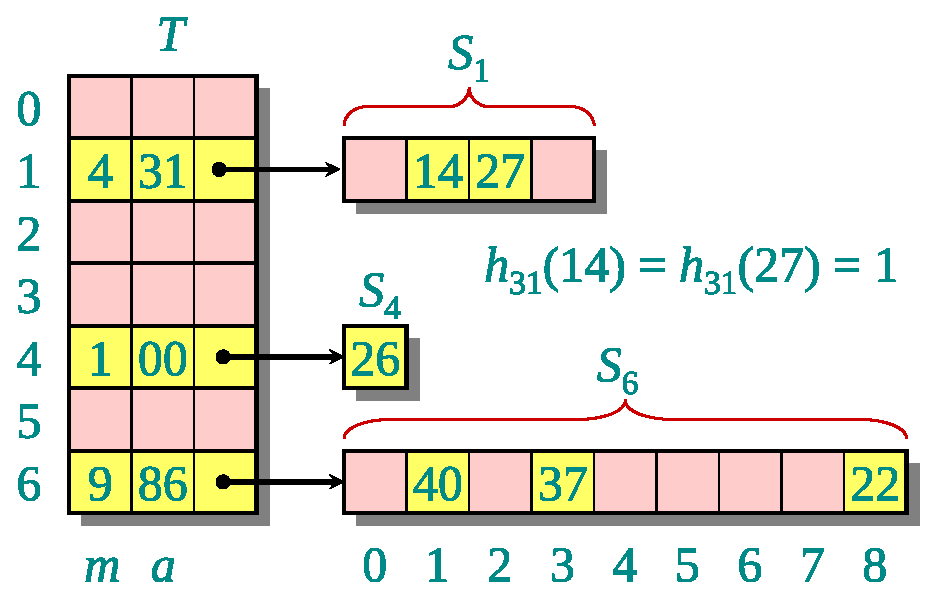
\includegraphics[width=3in]{lecture8/ideal.eps}
  \caption{Идеальное хэширование}
  \label{fig:ideal}
\end{figure}

$S_1, S_2, \twodots, S_m$ -- хэш-таблицы второго уровня, размер каждой из которых зависит от количества элементов $n_i$ попавших в слот $i$ таблицы $T$ и равен $m = n_i^2$. Каждая таблица $S_i$ обслуживается собственной хэш-функцией $h$ с индексом $a_i$ (вторая колонка таблицы $T$). Выбор функций происходит на этапе заполнения таблицы (предвычисление).

Теорема: пусть $H$ -- класс универсальных хэш-функций для таблицы размера $m = n^2$. Тогда для случайной функции $h \in H$ при хэшировании $n$ ключей ожидаемое количество коллизий не превышаеть $1/2$.

По свойству универсального множества, вероятность того, что два ключа дадут коллизию для функции $h$ равна $1/m = 1/n^2$. Т.к. всего существует $C_2^n$ пар ключей, ожидаемое количество коллизий равно
\begin{equation*}
  \frac{n!}{2!(n-2)!}\frac{1}{n^2} = \frac{n(n-1)}{2}\frac{1}{n^2} < \frac{1}{2}
\end{equation*}

Следствие: вероятность отсутствия коллизий составляет как минимум $1/2$.

Используя неравенство Маркова
\begin{equation*}
  Pr\{X \geqslant t\} \leqslant E[X]/t  
\end{equation*}
рассматривая случай для $t =1$, получим, что вероятность одной или более коллизий равна не более чем $1/2$.

Т.е. множество $H$ как минимум на половину состоит из функций, удовлетворяющих нашим требованиям.

\subsection{Анализ размера таблицы}

Для первого уровня хэш-таблицы $T$ используется $m=n$ ячеек. Пусть $n_i$ -- случайная величина, показывающая количество ключей, попавших в слот $i$ первого уровня таблицы $T$. Используя $n_i^2$ слотов для таблицы второго уровня $S_i$, ожидаемый общий размер для суммы двух уровней будет равен:
\begin{equation*}
  E\left[\sum_{i=0}^{m-1}\Theta(n_i^2)\right] = \Theta(n)
\end{equation*}

\end{document}
